\documentclass{article}
\newcommand{\exptitle}{QM Assignment}
\newcommand{\course}{PHYS3111 - Quantum Mechanics}

\usepackage{graphicx}
\usepackage{pgf}
\usepackage{lmodern}
\usepackage{import}
\usepackage{booktabs}
\usepackage{tabu}
\usepackage{float}
\usepackage[hidelinks]{hyperref}
\usepackage{amsmath}
\usepackage{amsfonts}
\usepackage[margin=1in]{geometry}
\usepackage{pythonhighlight}
\usepackage[toc]{appendix}
\usepackage{float}
\usepackage{placeins}
\usepackage{natbib}
\usepackage{lmodern}
\usepackage{subfig}
\usepackage[utf8]{inputenc}
\usepackage[T1]{fontenc}
\usepackage{upgreek}
\usepackage{chemmacros}
\usepackage{braket}
\usepackage{newpxtext,newpxmath}
\usepackage{tikz}

\DeclareMathOperator{\sech}{sech}
\DeclareMathOperator{\cosech}{cosech}

\setlength{\parskip}{1em}
\setlength{\parindent}{0em}

\begin{document}

\begin{titlepage}
    \begin{center}
        \vspace*{7cm}

        \Huge
        \textbf{\exptitle}

        \vspace{0.5cm}
        \LARGE
        \course

        \vspace{1.5cm}

        \textbf{Toby Nguyen - z5416116}
    \end{center}
\end{titlepage}

\tableofcontents


\section{Question 1 - Time Independent Perturbation Theory}

\subsection{Harmonic Oscillator}

We have a potential $V(x) = \frac{1}{2}kx^2$ with known energies $E_n=\hbar \omega (n+\frac{1}{2})$. The perturbation of the spring constant is $k\rightarrow k(1+\epsilon)$

\begin{enumerate}
    \item The Hamiltonian including the perturbation is given as $H = \frac{p^2}{2m}+\frac{1}{2}kx^2(1+\epsilon)$. Consider
    \begin{equation*}
        \omega = \sqrt{\frac{k}{m}}
    \end{equation*}
    including the pertubation, the new oscillating frequency becomes
    \begin{align*}
        \omega' &= \sqrt{\frac{k(1+\epsilon)}{m}} = \sqrt{\frac{k}{m}}\sqrt{1+\epsilon} \\
        &=\omega \sqrt{1 + \epsilon}.
    \end{align*}
    Here we can apply our second order expansion in $\epsilon$
    \begin{equation*}
        \sqrt{1+\epsilon} \approx 1 + \frac{\epsilon}{2} - \frac{\epsilon^2}{8} + O(\epsilon^3).
    \end{equation*}
    This leads us to an approximate new frequency 
    \begin{equation*}
        \omega' = \omega\left(1+\frac{\epsilon}{2}- \frac{\epsilon^2}{8}\right).
    \end{equation*}
    The new energy given by the perturbed oscillating frequency is then 
    \begin{equation*}
        E_{n} = \hbar \omega\left(n + \frac{1}{2}\right)\left(1+\frac{\epsilon}{2}- \frac{\epsilon^2}{8}\right)
    \end{equation*}
    which means our energy correction is then 
    \begin{equation} \label{eqn:1}
        \Delta E_{n}=\hbar \omega \left(n+\frac{1}{2}\right)\left(\frac{\epsilon}{2}- \frac{\epsilon^2}{8}\right)
    \end{equation}
    \item Begin with the Hamiltonian, $H'$,
    \begin{align*}
        H' &= H_0 + \lambda V \\
        &= \underbrace{\frac{p^2}{2m} + \frac{1}{2}kx^2}_\text{$H_0$} + \underbrace{\frac{1}{2}k\epsilon x^2}_\text{$\lambda V$}
    \end{align*}
    First order perturbation theory states that, with $\psi^{(0)}_n \approx \psi_n$ 
    \begin{equation}
        \Delta E^{(1)}_n = \lambda V_{nn} = \bra{\psi_n}\lambda V \ket{\psi_n}
    \end{equation}
    Plugging in our perturbation, and a known result for $\braket{x^2} = \frac{\hbar}{2m\omega}\left(2n+1\right)$
    \begin{align*}
        \Delta E^{(1)}_n &= \braket{\epsilon\frac{1}{2}kx^2} \\
        &= \frac{k\epsilon}{2}\braket{x^2} \\
        &= \frac{k\epsilon}{2}\frac{\hbar}{2m\omega}\left(2n+1\right) \\
        &= \hbar \omega \left(n + \frac{1}{2}\right)\frac{\epsilon}{2} \: \: \: \: \text{$\left(\omega = \sqrt{\frac{k}{m}}\right)$}.
    \end{align*}
    We find that our result is partially in Part 1, therefore the results deviate as we go up in orders.
\end{enumerate}

\subsection{General 2 Level System}
\begin{enumerate}
    \item The total Hamiltonian is hermitian if and only if $V_{ab} = V^{*}_{ba}$.
    \item Before we calculate the exact energies for this two level system. Let's consider a generic 2x2 hermitian matrix $M$, where M 
    satisfies our hermitian condition from Part 1.
    \begin{equation*}
        M = \begin{pmatrix}
            a & b \\ b^* & d
        \end{pmatrix}.
    \end{equation*}
    We will now calculate the eigenvalues, $\epsilon$, of this matrix, 
    \begin{align*}
        0 &= \left|H - \epsilon I\right| \\
        0 &= \begin{vmatrix}
            a-\epsilon & b \\ b^* & d-\epsilon
        \end{vmatrix} \\
        &= (a-\epsilon)(d-\epsilon)-|b|^2 \\
        &= \epsilon^2 -\epsilon(a+d)+ad - |b|^2 \\
        \epsilon_{\pm} &= \frac{(a+d)\pm\sqrt{(a+d)^2+4|b|^2-4ad}}{2} \\
        &= \frac{(a+d)\pm\sqrt{a^2+2ad+d^2-4ad+4|b|^2}}{2} \\
        &= \frac{(a+d)\pm\sqrt{(a-d)^2+4|b|^2}}{2}
    \end{align*}
    We can substitute $a=E^{(0)}_a + \lambda V_{aa}$, $b = \lambda V_{ab}$ and $d=E^{(0)}_{b}+ \lambda V_{bb}$ here to obtain our exact energies
    \begin{equation*}
        \epsilon_{\pm} = \frac{(E^{(0)}_a + E^{(0)}_b + \lambda(V_{aa}+V_{bb}))\pm\sqrt{(E^{(0)}_a - E^{(0)}_b + \lambda(V_{aa} - V_{bb}))^2+4V_{ab}^2}}{2}
    \end{equation*}
    \item Consider the expression before substitution from the last part, also consider 
    \begin{equation*}
        \sqrt{(a-d)^2+4|b|^2} = |a-d|\sqrt{1+\frac{4|b|^2}{(a-d)^2}}
    \end{equation*}
    Here we can apply our Taylor expansion of $\sqrt{(1+x)}\approx 1 + \frac{x}{2}$,
    \begin{equation*}
        |a-d|\sqrt{1+\frac{4|b|^2}{(a-d)^2}} \approx |a-d|\left(1+\frac{2|b|^2}{(a-d)^2}\right)
    \end{equation*}
    So our energy becomes 
    \begin{equation*}
        \epsilon_{\pm} = \frac{(a+d)\pm|a-d|\left(1+\frac{2|b|^2}{(a-d)^2}\right)}{2}.
    \end{equation*}
    Here we can make the same substitutions as before, but with now $\lambda = 1$ and also $E^{(0)}_b > E^{(0)}_a$ so 
    $|a-d| = d-a$,
    \begin{align*}
        \epsilon_{\pm} &= \frac{d+a}{2} \pm \frac{d-a}{2}\left(1+\frac{2|b|^2}{(d-a)^2}\right) \\
        &= \frac{d+a \pm (d-a)}{2} + \frac{|b|^2}{d-a}.
    \end{align*}
    For the first eigenvalue, $\epsilon_{-}$
    \begin{equation*}
        \epsilon_{-} = a + \frac{|b|^2}{d-a} = E^{(0)}_b + \lambda V_{bb} - \frac{\lambda^2|V_{ab}|^2}{E^{(0)}_b + \lambda V_{bb} - E^{(0)}_a - \lambda V_{aa}}
    \end{equation*}
    and our second eigenvalue $\epsilon_{+}$
    \begin{equation*}
        \epsilon_{+} = d + \frac{|b|^2}{d-a} = E^{(0)}_a + \lambda V_{aa} + \frac{\lambda^2|V_{ab}|^2}{E^{(0)}_b + \lambda V_{bb} - E^{(0)}_a - \lambda V_{aa}}
    \end{equation*}
    We have to treat the denominator using a geometric sum so consider $\Delta E = E^{(0)}_b - E^{(0)}_a$ and $\delta V = V_{aa} - V_{bb}$, then 
    \begin{equation*}
        \frac{1}{\Delta E - \lambda \delta V} = \frac{1}{\Delta E} \frac{1}{1-\lambda\frac{\delta V}{\Delta E}} = \frac{1}{\Delta E} \left(1+ 
        \lambda \frac{\delta V}{\Delta E} + O\left(\left(\frac{\delta V}{\Delta E}\right)^2\right)\right).
    \end{equation*}
    That second term in the brackets would contribute a $\lambda$ to the overall fraction with it already being $\lambda^2$ so we can disregard that term 
    and only take the sum equal to $\frac{1}{\Delta E}$. Now setting $\lambda = 1$,
    \begin{equation*}
        \epsilon_{-} = E^{(0)}_a + V_{aa} - \frac{|V_{ab}|^2}{E^{(0)}_b - E^{(0)}_a}
    \end{equation*}
    and 
    \begin{equation*}
        \epsilon_{+} = E^{(0)}_b + V_{bb} + \frac{|V_{ab}|^2}{E^{(0)}_b - E^{(0)}_a}.
    \end{equation*}
    These are the exact energies (up to order two), and so we can check the relationship $\Delta E^{(2)} = \epsilon_{\text{exact}}-E^{(0)}-\Delta E^{(1)}$.
    Given that second order perturbation theory predicts that $\Delta E^{(1)}_n = V_{nn}$ and 
    \begin{equation*}
        \Delta E^{(2)} = \sum_{m\neq n}\frac{|Vmn|^2}{E^{(0)}_n - E^{(0)}_m}.
    \end{equation*} 
    It is trivial to prove that the results obtained agree with perturbation theory, for example, take one of the eigenvalues,
    \begin{equation*}
        \underbrace{\epsilon_{-}}_{\text{Exact energy}} = \underbrace{E^{(0)}_a}_{\text{Zeroth order (no perturbation)}} + 
        \underbrace{V_{aa}}_{\text{First order}} + \underbrace{\frac{|V_{ab}|^2}{E^{(0)}_b - E^{(0)}_a}}_{\text{Second Order}}.
    \end{equation*}
    \item A requirement for our Taylor expansion of $\sqrt{(1+x)}$ to converge is that $|x| < 1$ so with $V_{aa} = V_{bb} = 0$,
    \begin{align*}
        \frac{4|b|^2}{(d-a)^2} &< 1 \\
        \left|\frac{V_{ab}}{E^{(0)}_b -E^{(0)}_a}\right| &< \frac{1}{2}.
    \end{align*}
\end{enumerate}

\subsection{Degenerate perturbation theory and the Hydrogen atom}
\begin{enumerate}
    \item Relativistic momentum is given as 
    \begin{equation*}
        p = \frac{mv}{\sqrt{1-\left(\frac{v}{c}\right)^2}}
    \end{equation*}
    and relativistic kinetic energy is given as 
    \begin{equation*}
        T = \frac{mc^2}{\sqrt{1-\left(\frac{v}{c}\right)^2}}-mc^2.
    \end{equation*}
    Consider the expression 
    \begin{align*}
        p^2c^2 + m^2c^4 &= \frac{m^2v^2c^2}{1-\frac{v^2}{c^2}} + m^2c^4 \\
        &= \frac{m^2v^2c^4}{c^2-v^2} + \frac{m^2c^4(c^2-v^2)}{c^2-v^2} \\
        &= \frac{m^2c^6}{c^2-v^2} \\
        &= \frac{m^2c^4}{1-\frac{v^2}{c^2}} \\
        &= (T+mc^2)^2
    \end{align*}
    Therefore we can obtain an alternative expression for the kinetic energy, $T$,
    \begin{align*}
        T &= \sqrt{[p^2c^2 + m^2c^4]} - mc^2 \\
        &= mc^2 \sqrt{1+\frac{p^2}{m^2c^2}}-mc^2.
    \end{align*}
    Using another Taylor expansion, this time taking only the term after our usual $\frac{p^2}{2m}$ (lowest order).
    \begin{equation*}
        T = mc^2\left(1+\frac{p^2}{2m^2c^2}-\frac{1}{8}\frac{p^4}{m^4c^4}+...\right)-mc^2 = \frac{p^2}{2m} - \frac{1}{8}\frac{p^4}{m^3c^2}.
    \end{equation*}
    The perturbed Hamiltonian is therefore 
    \begin{equation*}
        H' = -\frac{1}{8}\frac{p^4}{m^3c^2}.
    \end{equation*}
    The first order correction to energy, with the use of an operator trick (taken from Griffiths) can be written as 
    \begin{equation*}
        \Delta E^{(1)} = \braket{\psi | H' | \psi} = -\frac{1}{8m^3c^2}\braket{\psi | p^4 | \psi} = -\frac{1}{8m^3c^2}\braket{p^2 \psi | p^2 \psi}.
    \end{equation*}
    If we quickly to return to our non-relativistic/unperturbed Hamiltonian, we can obtain an expression for $p^2 \psi$, that is,
    \begin{align*}
        H_0 \psi &= E \psi \\
        \left(\frac{p^2}{2m} + V \right) \psi &= E \psi \\
        p^2 \psi &= 2m(E-V) \psi.
    \end{align*}
    Therefore the energy correction becomes, 
    \begin{equation*}
        \Delta E^{(1)} = -\frac{1}{8m^3c^2}4m^2\braket{(E-V)\psi^*(E-V)\psi}=-\frac{1}{2mc^2}\braket{(E-V)^2} = -\frac{1}{2mc^2}(E^2 - 2E\braket{V}
        +\braket{V^2}).
    \end{equation*}

    The expression $\braket{V}$ is known and was used in previous questions, $\braket{V} = \frac{1}{2}k\braket{x^2} = \frac{1}{2}k(2n+1)
    \frac{\hbar}{2m\omega} = \frac{\hbar\omega}{2}\left(n+\frac{1}{2}\right)$. We also know that $E=\hbar \omega \left(n+\frac{1}{2}\right)$

    The challenge is now obtaining an expression for $\braket{V^2}$, this next section is such, then dedicated to it. I'm not sure if there was a faster way
    to do this, such as computing $p^4\psi$ directly to obtain $\Delta E^{(1)}$ but I sought to find a better way, and eventually I found myself to deep to 
    not try it. So here is how I found $\braket{V^2}$ to complete the roundabout way.

    We know that $\braket{V^2}=\frac{1}{4}k\braket{x^4}$. The challenge is then to find $\braket{x^4}$. Consider the creation and annihilation ladder operators,
    \begin{equation*}
        x=\sqrt{\frac{\hbar}{2m\omega}}(\hat{a}+\hat{a}^{\dagger}).
    \end{equation*}
    These operators have the important characters $\left[\hat{a},\hat{a}^{\dagger}\right]=1$ and also for harmonic oscillators 
    \begin{align*}
        \hat{a}^{\dagger}\ket{n} &= \sqrt{n+1}\ket{n+1} \\
        \hat{a} \ket{n} &= \sqrt{n}\ket{n-1}.
    \end{align*}
    Our expression then becomes
    \begin{equation*}
        \braket{x^4} = \left(\frac{\hbar}{2m\omega}\right)^2\braket{(\hat{a}+\hat{a}^{\dagger})^4}.
    \end{equation*}
    We can sort of use the binomial expansion here, however note that because the two operators do not commute we can't just plug in the coefficients. Instead we 
    can expand this more smartly and succintly. Notice that the operators each either go up a rung or go down meaning if we have 
    \begin{equation*}
        \braket{n | (\hat{a}^{\dagger})^m\hat{a}^n|n}=0 \text{ where $m\neq n$}
    \end{equation*}
    then the term will go to zero as $\braket{n_+|n_-}=0$ if $n_+ \neq n_-$. Therefore the only non-zero terms in the expansion will be the one where 
    the powers of the two operators are equal, i.e the exponent of each is 2. By inspection or by binomial expansion rules, there will be 6 terms with this 
    quality so

    \begin{equation*}
        (\hat{a}+\hat{a}^{\dagger})^4 = 3\hat{a}^2 (\hat{a}^{\dagger})^2 + 3(\hat{a}^{\dagger})^2\hat{a}^2.
    \end{equation*}
    The second term is fine because we can use that in our calculation later but we need to flip the operators in the first term so consider 
    \begin{align*}
        \hat{a}^2(\hat{a}^{\dagger})^2 &= \hat{a}\hat{a}\hat{a}^{\dagger}\hat{a}^{\dagger} = \hat{a}(\hat{a}^{\dagger}\hat{a} + 1)\hat{a}^{\dagger} =
        \hat{a}\hat{a}^{\dagger}\hat{a}\hat{a}^{\dagger}+\hat{a}\hat{a}^{\dagger}= (\hat{a}^{\dagger}\hat{a}+1)(\hat{a}^{\dagger}\hat{a}+1)+(\hat{a}^{\dagger}\hat{a}+1) \\
        &= (\hat{a}^{\dagger} \hat{a})^2+2\hat{a}^{\dagger}\hat{a}+1+\hat{a}^{\dagger}\hat{a}+1 \\
        &= (\hat{a}^{\dagger} \hat{a})^2 + 3\hat{a}^{\dagger}\hat{a}+2 \\
        &= \hat{a}^{\dagger}\hat{a}\hat{a}^{\dagger}\hat{a}+ 3\hat{a}^{\dagger}\hat{a}+2 \\
        &= \hat{a}^{\dagger}(\hat{a}^{\dagger}\hat{a}+1)+ 3\hat{a}^{\dagger}\hat{a}+2 \\
        &= (\hat{a}^{\dagger})^2\hat{a}^2+\hat{a}^{\dagger}\hat{a}+ 3\hat{a}^{\dagger}\hat{a}+2 \\
        &= (\hat{a}^{\dagger})^2\hat{a}^2+ 4\hat{a}^{\dagger}\hat{a}+2
    \end{align*}
    Our expectation value is then 
    \begin{align*}
        \braket{(\hat{a}+\hat{a}^{\dagger})^4} &= 3(\braket{\hat{a}^2(\hat{a}^{\dagger})^2}+\braket{(\hat{a}^{\dagger})^2\hat{a}}) \\
        &= 3(\braket{(\hat{a}^{\dagger})^2\hat{a}+4\hat{a}^{\dagger}\hat{a}+2}+\braket{(\hat{a}^{\dagger})^2\hat{a}}) \\
        &= 3(2\braket{(\hat{a}^{\dagger})^2\hat{a}}+4\braket{\hat{a}^{\dagger}\hat{a}}+2) \\
        &= 3(2n(n-1)+4n+2) \\
        &= 6n^2+6n+3
    \end{align*}
    Finally back to our objective,
    \begin{align*}
        \braket{V^2} &= \frac{1}{4}k^2(6n^2+6n+3)\left(\frac{\hbar}{2m\omega}\right)^2 \\
        &= \frac{1}{16}\hbar^2\omega^2(6n^2+6n+3)
    \end{align*}
    Plugging all this into our expression for the lowest order relativistic energy correction for the harmonic oscillator,
    \begin{align*}
        \Delta E^{(1)} &= -\frac{1}{2mc^2}\left(E^2 - 2E\braket{V}+\braket{V^2}\right) \\
        &= -\frac{1}{2mc^2}\left(\hbar^2\omega^2\left(n+\frac{1}{2}\right)^2-2\times\frac{1}{2}\hbar^2\omega^2\left(n+\frac{1}{2}\right)^2
        +\frac{\hbar^2\omega^2}{16}(6n^2+6n+3)\right) \\
        &= -\frac{1}{2mc^2}\left(\frac{\hbar^2\omega^2}{16}(6n^2+6n+3)\right) \\
        &= -\frac{1}{2mc^2}\left(\frac{3\hbar^2\omega^2}{8}\left(n^2+n+\frac{1}{2}\right)\right) \\
        &= -\frac{1}{2mc^2}\left(\frac{3\hbar^2\omega^2}{8}\left(\left(n+\frac{1}{2}\right)^2+\frac{1}{4}\right)\right) \\
        &= -\frac{1}{2mc^2}\left(\frac{3}{8}E_n^2 + \frac{3E_n^2}{32\left(n+\frac{1}{2}\right)^2}\right) \\
        &= -\frac{E^2_n}{2mc^2}\left(\frac{3}{8}+\frac{3}{32\left(n+\frac{1}{2}\right)^2}\right)
    \end{align*}
    \item We can get the fine structure formula from adding the relativistic correction formula to the spin-orbit coupling formula, that is, we 
    can obtain 
    \begin{align*}
        E^{(1)}_{FS}&=E^{(1)}_r+E^{(1)}_{SO} \\
        &= -\frac{E_n^2}{2mc^2}\left(\frac{4n}{l+\frac{1}{2}-3}\right) + n\frac{E_n^2}{mc^2}\left(\frac{j(j+1)-l(l+1)-\frac{3}{4}}{l
        (l+\frac{1}{2})(l+1)}\right).
    \end{align*}
    We know that $j= l\pm \frac{1}{2}$ when $l=neq 0$ and $j=l + \frac{1}{2}$ when $l=0$. So we have to find the formula for both $+$ and $-$, 
    however, as we will soon find, both expressions are equivalent.
    For the $j=l + \frac{1}{2}$ case, so $l=j-\frac{1}{2}$, the right hand side of the equation is then 
    \begin{equation*}
        RHS = \frac{E_n^2}{2mc^2}\left(3-\frac{4n}{j}+2n\left(\frac{j(j+1)-(j-\frac{1}{2})(j+\frac{1}{2})-\frac{3}{4}}{(j-\frac{1}{2})j(
        j+\frac{1}{2})}\right)\right)
    \end{equation*}
    The numerator of the big fraction,
    \begin{equation*}
        j(j+1)-(j-\frac{1}{2})(j+\frac{1}{2})-\frac{3}{4} = j^2 + j - j^2 + \frac{1}{4}-\frac{3}{4} = j-\frac{1}{2}
    \end{equation*}
    We can see this cancels with the factor in the denominator so that big fraction becomes $\frac{2n}{j(j+\frac{1}{2})}$.
    \begin{align*}
        RHS &= \frac{E_n^2}{2mc^2}\left(3-\frac{4n}{j}+\frac{2n}{j(j+\frac{1}{2})}\right) \\
        &= \frac{E^2_n}{2mc^2}\left(3-\frac{4n}{j}+\frac{4n}{j}-\frac{4n}{j+\frac{1}{2}}\right) \\
        &= \frac{E_n^2}{2mc^2}\left(3-\frac{4n}{j+\frac{1}{2}}\right)
    \end{align*}
    Here we used a sweet trick where $\frac{4n}{j}-\frac{4n}{j+\frac{1}{2}}=\frac{4n(j+\frac{1}{2}-4nj)}{j(j+\frac{1}{2})}=\frac{2n}{j(j+\frac{1}{2})}$.
    For the $j=l-\frac{1}{2}$ case, meaning $l=j+\frac{1}{2}$,
    \begin{equation*}
        RHS = \frac{E_n^2}{2mc^2}\left(3-\frac{4n}{j+1}+2n\left(\frac{j(j+1)-(j+\frac{1}{2})(j+\frac{3}{2})-\frac{3}{4}}{(j+\frac{1}{2})
        (j+1)(j+\frac{3}{2})}\right)\right).
    \end{equation*}
    Let us inspect the numerator again,
    \begin{equation*}
        j(j+1)-(j+\frac{1}{2})(j+\frac{3}{2})-\frac{3}{4} = j^2+j-j^2-\frac{3}{2}j-\frac{1}{2}j-\frac{3}{4}-\frac{3}{4} = - j -\frac{3}{2}
    \end{equation*}
    Again, this will cancel with the $j+\frac{3}{2}$ factor on the denominator, so the fraction becomes $\frac{2n}{(j+\frac{1}{2})(j+1)}$, 
    using the same trick i.e $\frac{2n}{(j+\frac{1}{2})(j+1)}=\frac{4n}{j+\frac{1}{2}}-\frac{4n}{j+1}$.
    \begin{align*} 
        RHS &= \frac{E_n^2}{2mc^2}\left(3-\frac{4n}{j+1}-\frac{2n}{(j+\frac{1}{2})(j+1)}\right) \\
        &= \frac{E_n^2}{2mc^2}\left(3-\frac{4n}{j+1}+\frac{4n}{j+1}-\frac{4n}{j+\frac{1}{2}}\right) \\
        &= \frac{E_n^2}{2mc^2}\left(3-\frac{4n}{j+\frac{1}{2}}\right)
    \end{align*}
    This agrees with the other case and the given fine structure formula.
    \item Bohr theory states that the energy of an electron in the nth shell is $E_n = -\frac{R_y}{n^2}$, therefore 
    \begin{equation*}
        \Delta E = R_y\left(\frac{1}{n_f^2}-\frac{1}{n_i^2}\right).
    \end{equation*}
    The transition then has energy $13.6eV \times (\frac{1}{2^2}-\frac{1}{3^2})=13.6eV \times \frac{5}{36} \approx 1.89 eV$. Using $E=hf$ and 
    $c=f\lambda$, we can obtain the frequency $4.567 \times 10^{14}$ Hz and the wavelength $656.4$ nm.

    To determine the line spacing and their value by the fine structure splitting, we first consider the electric dipole selection rules. That 
    is, only transitions of $\Delta l = \pm 1$ and $\Delta m=0, \pm 1$ are allowed, derived from the spherical harmonics of the wavefunctions 
    in the hydrogen atom. Visually, the allowed transitions can be shown in the Figure below,

    \begin{center}
    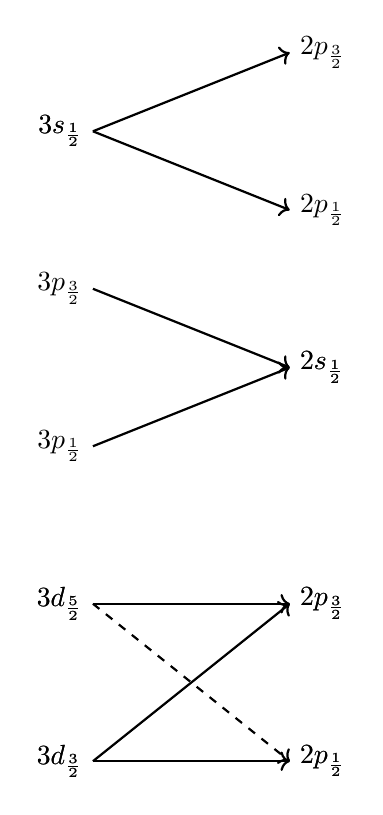
\begin{tikzpicture}
        \draw[thick,->] (0,0) node [anchor=east] {$3s_{\frac{1}{2}}$} to (2.5,1) node [anchor=west] {$2p_{\frac{3}{2}}$};
        \draw[thick,->] (0,0) node [anchor=east] {$3s_{\frac{1}{2}}$} to (2.5,-1) node [anchor=west] {$2p_{\frac{1}{2}}$};
        \draw[thick,->] (0,-2) node [anchor=east] {$3p_{\frac{3}{2}}$} to (2.5,-3) node [anchor=west] {$2s_{\frac{1}{2}}$};
        \draw[thick,->] (0,-4) node [anchor=east] {$3p_{\frac{1}{2}}$} to (2.5,-3) node [anchor=west] {$2s_{\frac{1}{2}}$};
        \draw[thick,->] (0,-6) node [anchor=east] {$3d_{\frac{5}{2}}$} to (2.5,-6) node [anchor=west] {$2p_{\frac{3}{2}}$};
        \draw[thick,->,dashed] (0,-6) node [anchor=east] {$3d_{\frac{5}{2}}$} to (2.5,-8) node [anchor=west] {$2p_{\frac{1}{2}}$};
        \draw[thick,->] (0,-8) node [anchor=east] {$3d_{\frac{3}{2}}$} to (2.5,-6) node [anchor=west] {$2p_{\frac{3}{2}}$};
        \draw[thick,->] (0,-8) node [anchor=east] {$3d_{\frac{3}{2}}$} to (2.5,-8) node [anchor=west] {$2p_{\frac{1}{2}}$};
    \end{tikzpicture}
    \end{center}
    The dashed arrow indicates a forbidden transition, one of many not shown in the diagram. Therefore, there are only 7 possible transitions 
    but some are degenerate. If we look at the energy due to fine splitting formula, we see that it depends on $j$ and $n$, so if we look at the 
    figure above, lets consider our $(n,j)$ pairs. By inspection we only have $(3,\frac{1}{2}) \rightarrow (2,\frac{3}{2})$, $(3,\frac{3}{2})
    \rightarrow (2,\frac{1}{2})$ and $(3,\frac{1}{2})\rightarrow (2,\frac{1}{2})$, which is expected as $\Delta j$ can only take on values of 
    $0, \pm 1$. Therefore, the original red Balmer line is split into 3 lines, each with energies, -8.79 $\mu$eV, 3.64 $\mu$eV and 4.98 $\mu$eV.
\end{enumerate}

\subsection{Feynman-Hellman Theorem}
We are required to prove the Feynman-Hellmann theorem, that is 

\begin{enumerate}
    \item \begin{align*}
        \text{RTP } \frac{\partial E_n}{\partial \lambda} &= \braket{\psi_n | \frac{\partial H}{\partial \lambda} | \psi_n} \\
        LHS &= \frac{\partial}{\partial \lambda}\braket{\psi_n | H | \psi_n} \\
        &= \int_{-\infty}^{\infty}\frac{\partial}{\partial \lambda}\left(\psi_n^* H \psi_n \right)dx \\
        &= \int_{-\infty}^{\infty}\frac{\partial}{\partial \lambda}\left(\psi_n^*H\right)\psi + \psi^*_n H 
        \frac{\partial}{\partial \lambda}\psi dx \\
        &= \int_{-\infty}^{\infty}\frac{\partial}{\partial \lambda}\psi_n^* H \psi + \psi^* \frac{\partial}{\partial \lambda} H \psi 
        \psi^* H \frac{\partial}{\partial \lambda} \psi dx \\
        &= \braket{\frac{\partial}{\partial \lambda} \psi_n | H | \psi_n} + \braket{\psi_n | H | \frac{\partial}{\partial \lambda} 
        \psi_n} + \braket{\psi_n | \frac{\partial H}{\partial \lambda}| \psi_n} \\
        &= E \braket{\frac{\partial}{\partial \lambda} \psi_n | \psi_n} + E \braket{\psi_n | \frac{\partial}{\partial \lambda}
        \psi_n} + \braket{\psi_n | \frac{\partial H}{\partial \lambda} | \psi_n} \\
        &= E \frac{\partial}{\partial \lambda} \braket{\psi_n | \psi_n} + E \frac{\partial}{\partial \lambda} \braket{\psi_n | \psi_n}
        + \braket{\psi_n | \frac{\partial H}{\partial \lambda} | \psi_n} \\
        &= \braket{\psi_n | \frac{\partial H}{\partial \lambda} | \psi_n} \\
        &= RHS \\
        &\therefore \text{ QED.}
    \end{align*}
    \item We know that $E_n = \hbar \omega (n + \frac{1}{2})$ and $H = \frac{p^2}{2m}+\frac{1}{2}m \omega^2 x^2$. 
    i. Using $\lambda = \omega$, 
    \begin{align*}
        \frac{\partial E_n}{\partial \omega} &= \braket{\frac{\partial}{\partial \omega}\left(\frac{p^2}{2m}+
        \frac{1}{2}m\omega^2x^2\right)} \\
        \hbar\left(n+\frac{1}{2}\right)&=\braket{m\omega x^2} \\
        \frac{\hbar \omega}{2}\left(n+\frac{1}{2}\right)&=\braket{\frac{1}{2}m\omega^2 x^2} = \braket{V}
    \end{align*}
    ii. Using $\lambda = \hbar$,
    \begin{align*}
        \frac{\partial E_n}{\partial \hbar} &= \braket{\frac{\partial}{\partial \hbar}\left(-\frac{\hbar^2}{2m}\frac{d^2}{dx^2}+\frac{1}{2}
        m\omega^2x^2\right)} \\
        \omega\left(n+\frac{1}{2}\right) &= \braket{-\frac{\hbar}{m}\frac{d^2}{dx^2}} \\
        \frac{\hbar \omega}{2}\left(n+\frac{1}{2}\right) &= \braket{-\frac{\hbar^2}{2m}\frac{d^2}{dx^2}} = \braket{T}
    \end{align*}
    iii. Using $\lambda = m$,
    \begin{align*}
        \frac{\partial E_n}{\partial m} &= \braket{\frac{\partial}{\partial m}\left(\frac{p^2}{2m}+\frac{1}{2}m\omega^2 x^2\right)} \\
        0 &= \braket{-\frac{p^2}{2m^2}+\frac{1}{2}\omega^2x^2} \\
        &= -\frac{1}{m}\braket{T}+\frac{1}{m}\braket{V} \\
        \braket{T} &= \braket{V}.
    \end{align*}
    Here we assume $\omega$ is independent of $m$, if we didn't and so $\frac{\partial E_n}{\partial m} \neq 0$, but if we accounted for this, 
    we would still get the same relationship.
\end{enumerate}
\section{Question 2 - Variational Principle}

To find the best bound on $E_{gs}$, we start with the trial wavefunction of the form, 

\begin{equation*}
    \psi(x) = \frac{A}{x^2+b^2}
\end{equation*}

We first check that this wavefunction obeys boundary conditions, such as, as $x$ goes to infinity, the wavefunction should go to zero i.e 
\begin{align*}
    \lim_{x\rightarrow \pm \infty}\psi(x) &= 0 \\
    LHS &= \lim_{x\rightarrow \pm \infty}\frac{A}{x^2+b^2} \\
    &= \frac{A}{\infty}\\
    &= 0
\end{align*}
So it satisfies the boundary conditions. We know the wavefunction is normalised, so we can find $A$,

\begin{align*}
    \braket{\psi | \psi} &= 1 \\
    1 &= A^2 \int_{-\infty}^{\infty}\frac{1}{x^2+b^2}dx
\end{align*}

To find this integral, we need to make a substitution, let $x=b\tan{\theta}$ so $dx = b\sec^2{\theta}d\theta$,
\begin{equation*}
    \int \frac{1}{\left(b^2\left(\tan^2{\theta}+1\right)\right)^2}b\sec^2{\theta}d\theta = \frac{1}{b^3}\int\frac{1}{\sec^2{\theta}}d\theta 
\end{equation*}
Here, to resolve the bounds, we exploit the $tan\theta$ function, if the bounds are $-\infty$ to $\infty$, we have our new bounds $-\frac{\pi}{2}$
to $\frac{\pi}{2}$. So

\begin{align*}
    \frac{1}{b^3}\int_{-\frac{\pi}{2}}^{\frac{\pi}{2}}\cos^2{\theta}d\theta &= \frac{1}{b^3}\int_{-\frac{\pi}{2}}^{\frac{\pi}{2}}\frac{\cos{2\theta}+1}{2}d\theta \\
    &= \frac{1}{b^3}\left[\frac{\sin{2\theta}}{4}+\frac{\theta}{2}\right]^{\frac{\pi}{2}}_{-\frac{\pi}{2}} \\
    &= \frac{1}{b^3}\left[\frac{\pi}{4}+\frac{\pi}{4}\right] \\ 
    &= \frac{\pi}{2b^3}
\end{align*}

Therefore, $A^2 = \frac{2b^3}{\pi}$. Now to find energy as a function of $b$, we need to find the energy of the one-dimensional harmonic oscillator,
that is 

\begin{align*}
    E &= \braket{\psi | H | \psi} \\
    &= \braket{\psi | \frac{p^2}{2m}+\frac{1}{2}m\omega^2 x^2 | \psi} \\
    &= \braket{\psi | -\frac{\hbar^2}{2m}\frac{d}{dx^2} | \psi} + \braket{\psi | \frac{1}{2}m\omega^2 x^2 | \psi}
\end{align*}

Our challenge here is to find the second derivative of the wavefunction to get the expression for the momentum operator, so consider 

\begin{align*}
    \frac{d^2}{dx^2}\ket{\psi} &= \frac{d}{dx}\frac{d}{dx}\left(\frac{A}{x^2+b^2}\right) = \frac{d}{dx}\left(-\frac{2xA}{\left(x^2+b^2\right)^2} 
    \right) = -2A \frac{d}{dx}\left(\frac{x}{\left(x^2+b^2\right)^2}\right) \\
    &= -2A \left[\frac{(x^2+b^2)^2-x\times 2 \times 2x(x^2+b^2)}{(x^2+b^2)^4}\right] \\
    &= -2A \left[\frac{x^2+b^2-4x^2}{(x^2+b^2)^4}\right] \\
    &= -2A \left[\frac{-3x^2+b^2}{(x^2+b^2)^3}\right] \\
    \braket{\psi | -\frac{\hbar^2}{2m}\frac{d^2}{dx^2} | \psi} &=  \frac{\hbar^2 A^2}{m}\int_{-\infty}^{\infty}\frac{-3x^2+b^2}{(x^2+b^2)^4}dx \\
    \braket{\psi | \frac{1}{2}m\omega^2 x^2 | \psi} &= \frac{1}{2}m\omega^2 A^2 \int_{-\infty}^{\infty} \frac{x^2}{(x^2+b^2)^2}dx \\
    E &= \frac{\hbar^2 A^2}{m}\times \frac{\pi}{8b^5}+\frac{1}{2}m\omega^2A^2 \times \frac{\pi}{2b} \\
    &= \frac{\hbar^2}{2m}\frac{1}{2b^2}+\frac{1}{2}m\omega^2b^2 \\
\end{align*}

To find the best bound on $E_{gs}$, we need to minimise $E(b)$, so 

\begin{align*}
    \frac{\partial E}{\partial b} = 0 &= -\frac{\hbar^2}{2m}\frac{1}{b^3}+m\omega^2 b \\
    b&=\left(\frac{\hbar}{\sqrt{2}m\omega}\right)^{\frac{1}{2}}
\end{align*}

The minimum energy, i.e the lowest bound is 

\begin{align*}
    E_{\text{min}}&=\frac{\hbar^2}{2m}\frac{\sqrt{2}m\omega}{2\hbar}+\frac{1}{2}m\omega^2\frac{\hbar}{\sqrt{2}m\omega} \\
    &= \frac{\hbar \omega \sqrt{2}}{4}+\frac{\hbar \omega}{2\sqrt{2}} \\
    &= \frac{\hbar \omega}{2}\sqrt{2}.
\end{align*}

As expected, this is bigger than the exact ground state $E_{gs}=\frac{\hbar \omega}{2}$.

\section{Question 3 - WKB approximation}
We know that for a one dimensional potential, and in a classical allowed region $b \leq x \leq a$, we have the quantisation condition 
\begin{equation*}
    \int_{x_1}^{x_2}p(x)dx = \left(n-\frac{1}{2}\right)\pi \hbar
\end{equation*}
We need to find an expression for the integral, begin with momentum which can be represented as 

\begin{align*}
    p(x) &= \sqrt{2m(E-V(x))} \\
    &= \sqrt{2m(E-\alpha|x|^{\nu})} 
\end{align*}

We can exploit the even function of $V(x)$, this leads to $p(x)$ being also even, $x_1$ and $x_2$ are found when $E \approx V$ so we can 
say $p(x_1) = p(x_2)$.

\begin{align*}
    \int_{x_1}^{x_2}\sqrt{2m(E-\alpha|x|^{\nu})}dx &= 2\int_0^{x_2}\sqrt{2m(E-\alpha x^{\nu})}dx \\
    &= 2\sqrt{2mE}\int_{0}^{x_2}\sqrt{1-\frac{\alpha}{E}x^\nu}dx.
\end{align*}

To solve this integral, we need to know a few things, the first thing is to define $E = V(x_2) = \alpha x_{2}^{\nu}$ and then look at the 
beta function,

\begin{equation*}
    \beta(x,y) = \int_{0}^{1}t^{x-1}(1-t)^{y-1}dt = \frac{\Gamma(x)\Gamma(y)}{\Gamma(x+y)}.
\end{equation*}

To turn the integral we have into a beta function, we can use a substitution $z=\frac{\alpha}{E}x^{\nu}$ and so 
\begin{align*}
    x&=\left(\frac{Ez}{\alpha}\right)^{\frac{1}{\nu}} \\
    dx &= \left(\frac{E}{\alpha}\right)\frac{1}{\alpha}z^{\frac{1}{\nu}-1}dz
\end{align*}

Our integral then becomes 
\begin{align*}
    2\sqrt{2mE}\int_{0}^{x_2}\sqrt{1-\frac{\alpha}{E}x^\nu}dx &= 2\sqrt{2mE}\int_{0}^{1}(1-z)^{\frac{1}{2}}\left(\frac{E}{\alpha}\right)^\frac{1}{\nu}
    \frac{1}{\nu}z^{\frac{1}{\nu}-1}dz \\
    &= \frac{2\sqrt{2mE}}{\nu}\left(\frac{E}{\alpha}\right)^{\frac{1}{\nu}}\int_{0}^{1}(1-z)^{\frac{3}{2}}z^{\frac{1}{\nu}-1}dz
\end{align*}

Here, $y=\frac{3}{2}$ and $x=\frac{1}{\nu}$, so using our beta function

\begin{align*}
    \frac{2\sqrt{2mE}}{\nu}\left(\frac{E}{\alpha}\right)^{\frac{1}{\nu}}\beta\left(\frac{1}{\nu},\frac{3}{2}\right) &= 
    \frac{2\sqrt{2mE}}{\nu}\left(\frac{E}{\alpha}\right)^{\frac{1}{\nu}} \frac{\Gamma(\frac{1}{\nu})\Gamma(\frac{3}{2})}{\Gamma\left(\frac{1}{\nu}
    +\frac{3}{2}\right)} \\
    &= \left(n+\frac{1}{2}\right)\pi \hbar
\end{align*}

Now we solve for $E$,

\begin{align*}
    E^{\frac{1}{\nu}+\frac{1}{2}}&=\left(n-\frac{1}{2}\right)\pi\hbar\left[\frac{\Gamma\left(\frac{1}{\nu}+\frac{3}{2}\right)}{\Gamma\left(
    \frac{1}{\nu}\right)\sqrt{\pi}}\frac{\alpha^{\frac{1}{\nu}\nu}}{\sqrt{2m}}\right] \\
    E &= \alpha \left[\left(n-\frac{1}{2}\right)\hbar\frac{\Gamma\left(\frac{1}{\nu}+\frac{3}{2}\right)}{\Gamma\left(\frac{1}{\nu}+1\right)}
    \sqrt{\frac{\pi}{2m\alpha}}\right]^{\frac{2\nu}{2+\nu}}.
\end{align*}

\section{Question 4 - Scattering Theory}

\subsection{Rutherford Scattering}

\begin{figure} [H]
    \centering
    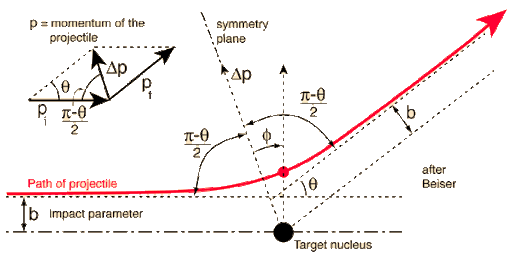
\includegraphics[width=0.7\textwidth]{unnamed.png}
    \caption{Path of projectile repelled by a Coulomb force}
    \label{fig:rscatter}
\end{figure}

Consider a projectile travelling along the $z$ axis in Figure \ref{fig:rscatter}, a distance $b$ away in the $x$ direction. 
There is a Coulomb interaction/force pushing the projectile away in the $x-z$ plane. We are going to assume that the impulse 
is directed in a straight line.

\begin{enumerate}
    \item  Here we have a displacement vector $r(t) = (b,0,vt)$. The distance from the target nucleus and the projectile is $r$ and 
        so the Coulomb force in the $x$ direction is given as 
        \begin{equation*}
            F_x(t) = \frac{1}{4\pi \epsilon_0}\frac{q_1q_2}{r^2}\cdot \hat{r}_x = \frac{k}{r^2}\cdot \hat{r}_x
        \end{equation*}

        The magnitude of this force is then 

        \begin{equation*}
            |F_x| = \frac{k}{r^3}\cdot b = \frac{kb}{(b^2+v^2t^2)^{\frac{3}{2}}}
        \end{equation*}

        We can now consider the impulse in the $x$ direction, $p_{\perp}$ where the $x$ direction is perpendicular to our $z$ 
        axis,

        \begin{align*}
            \Delta p_{\perp} &= \int_{-\infty}^{\infty}F_x(t)dt \\
            &= kb \int_{-\infty}^{\infty} \frac{dt}{(b^2+v^2t^2)^{\frac{3}{2}}}\\
            &= \frac{2k}{vb}
        \end{align*}

        Now we consider the geometry of the problem to find another representation for $\Delta p_{\perp}$. We will apply the 
        cosine rule to the triangle with $p_i$, $p_f$ and $\Delta p$, note that $|p_i| = |p_f|$ so that 

        \begin{align*}
            |\Delta p|^2 &= 2p^2 - 2p^2\cos{\theta} \\
            &= 2p^2(1-\cos\theta) \\
            &= 4p^2\left(\sin^2\frac{\theta}{2}\right) \\
            \Delta p &= 2p\sin{\frac{\theta}{2}}
        \end{align*}

        Then we have $\Delta p_{\perp} = \Delta p \cos{\frac{\theta}{2}} = p\sin{\theta}$. Now we apply small approximations, 
        assuming because the particle is heavy, there is a small deflection, $\sin{\theta} \approx 2\tan{\frac{\theta}{2}}$ so we finally have,

        \begin{align*}
            p\sin{\theta} &= \frac{2k}{vb} \\
            \frac{k}{b} &= \frac{1}{2}mv^2 \times 2 \tan{\frac{\theta}{2}} \\
            b &= \frac{k}{2E}\cot{\frac{\theta}{2}} \\
            &= \frac{q_1 q_2}{8\pi \epsilon_0 E}\cot{\frac{\theta}{2}}
        \end{align*}
    \item We know that 
    \begin{equation*}
        D(\theta) = \frac{b}{\sin{\theta}}\left|\frac{db}{d\theta}\right|.
    \end{equation*}
    Let's first find an expression for $\left|\frac{db}{d\theta}\right|$, starting with our result from 1.,
    \begin{align*}
        b&= \frac{q_1 q_2}{8\pi \epsilon_0 E}\cot{\frac{\theta}{2}}\\
        \frac{db}{d\theta} &= -\frac{q_1q_2}{16\pi\epsilon_0E}\text{cosec}^2{\frac{\theta}{2}}
    \end{align*}
    Plugging it into the $D(\theta)$ equation, applying small angle approximations $\cos{\frac{\theta}{2}}\approx 1$ and 
    $\sin{\theta}=2\sin{\frac{\theta}{2}}\cos{\frac{\theta}{2}} \approx 2\sin{\frac{\theta}{2}}$. 

    \begin{align*}
        D(\theta) &= \frac{q_1q_2}{8\pi \epsilon_0 E}\cot{\frac{\theta}{2}}\frac{1}{\sin{\theta}}\frac{q_1q_2}{16\pi 
        \pi\epsilon_0 E} \text{cosec}^2{\frac{\theta}{2}} \\ 
        &= \left(\frac{q_1 q_2}{16 \pi \epsilon_0 E} \frac{1}{\sin{\frac{\theta}{2}}}\right)^2
    \end{align*}
    \item The total cross section is found by 
    \begin{equation*}
        \sigma = \int D(\theta)d\Omega
    \end{equation*}
    where $\int d\Omega$ is the integral over solid angles. We can easily compute this,
    \begin{align*}
        \sigma &= \int_{0}^{2\pi}\int_{0}^{\pi}D(\theta)\sin{\theta}d\theta d\phi \\
        &= 2\pi \left(\frac{q_1 q_2}{16\pi \epsilon_0 E}\right)^2 \int_{0}^{\pi}\frac{\sin{\theta}}{\sin^4{\frac{\theta}{2}}}d\theta \\
        &= 4\pi \left(\frac{q_1 q_2}{16\pi \epsilon_0 E}\right)^2 \int_{0}^{\pi}\frac{\cos{\frac{\theta}{2}}}{\sin^3{\frac{\theta}{2}}}d\theta \\
        &= 4\pi \left(\frac{q_1 q_2}{16\pi \epsilon_0 E}\right)^2 \left[\text{cosec}^2\frac{\theta}{2}\right]^{\pi}_0
    \end{align*}
    We can see here that $\text{cosec}^2{0} \rightarrow \infty$ and then $\sigma \rightarrow \infty$.
\end{enumerate}

\subsection{Born Approximation}
The Born Approximation, we let $\psi \approx e^{-ikr}$ and so 
\begin{align*}
    f(k_i,k_f) &= -\frac{m}{2\pi\hbar^2}\int\psi^*V(r)\psi d^3r \\
    &= -\frac{m}{2\pi\hbar^2}\int e^{-ik_f\cdot r} V(r)e^{ik_i\cdot r} d^3r \\
    f(\Delta k) &= -\frac{m}{2\pi\hbar^2}\int V_0 e^{-\mu\frac{r^2}{a^2}}e^{-i\Delta k\cdot r}d^3 \: \: \: \: \text{where} \: \: \Delta k=k_f - k_i \\
    &= -\frac{m}{2\pi\hbar^2} V_0\times \frac{\pi^{\frac{3}{2}}a^3e^{-\frac{a^2\Delta k^2}{4\mu}}}{\mu^{\frac{3}{2}}} \\ 
    &= -\frac{a^3 m}{2\hbar^2}V_0 \sqrt{\frac{\pi}{\mu^3}}e^{-\frac{a^2\Delta k^2}{4\mu}}
\end{align*}
Using the same geometry as before, where $|k_i| = |k_f|$, we find that $\Delta k^2 = 2k^2(1-\cos{\theta})$ so 

\begin{equation*}
    f(\theta) = -\frac{a^3m}{2\hbar^2}V_0 \sqrt{\frac{\pi}{\mu^3}}e^{-\frac{a^2 2k^2(1-\cos\theta)}{4\mu}}
\end{equation*}

We know that 

\begin{equation*}
    \frac{d\sigma}{d\Omega} = |f(\theta)|^2 = \left(\frac{a^3m}{2\hbar^2}V_0\right)^2\frac{\pi}{\mu^3}e^{-\frac{a^2 2k^2(1-\cos\theta)}{4\mu}}
\end{equation*}

Now, the total cross section area is 

\begin{align*}
    \sigma &= \left(\frac{a^3m}{2\hbar^2}V_0\right)^2\frac{\pi}{\mu^3}\int{e^{-\frac{a^2 2k^2(1-\cos\theta)}{4\mu}}}d\Omega \\
    &= \left(\frac{a^3m\pi}{\hbar^2}V_0\right)^2\frac{1}{2\mu^3}e^{-\frac{a^2 2k^2}{4\mu}}\int_0^{\pi}e^{\frac{a^2 2k^2\cos{\theta}}{4\mu}}\sin{\theta}d\theta
\end{align*}

Let $u=-cos\theta$ so $du=\sin\theta d\theta$,

\begin{align*}
    \int_{0}^{\pi}e^{-\frac{a^2k^2\cos\theta}{4\mu}}\sin\theta d\theta &= \int_{-1}^{1}e^{-\frac{a^2k^2}{4\mu}u}du \\
    &= \left[-\frac{4\mu}{a^2k^2}e^{-\frac{a^2 k^2}{4\mu}u}\right]_{-1}^{1} \\
    &= \frac{4\mu}{a^2 k^2}\left(-e^{-\frac{a^2 k^2}{4\mu}}+e^{\frac{a^2 k^2}{4\mu}}\right)
\end{align*}

So our total cross section is, with $p=\hbar k$ and $E = \frac{p^2}{2m}$,

\begin{equation*}
    \sigma = \left(\frac{a^2\pi V_0}{\hbar}\right)^2\frac{1}{\mu^2 E}\left(1-e^{-\frac{-a^2 k^2}{2\mu}}\right).
\end{equation*}

Born approximation is valid so long as 

\begin{equation*}
    \left|\frac{2m}{\hbar^2k}\int_{0}^{\infty}drrV(r)\sin{kr}\right| \ll 1.
\end{equation*}

In the case of our Gaussian potential, this means that the Born approximation applies only for 

\begin{equation*}
    \frac{mV_0}{\hbar^2k}\left(\frac{a}{\sqrt{\mu}}\right)^2 \ll 1.
\end{equation*}

\section{Question 5 - Time Dependent Perturbation Theory}
\begin{enumerate}
    \item There is the ground state $n=1$, $\ket{100}$ and then quadruply degenerate states $n=2$, $\ket{200}, \ket{210}, 
    \ket{211}$ and $\ket{21 -1}$, where a state is denoted $\ket{njm}$. To find the four matrix elements $H'_{ij}$, we 
    will compute $\braket{\psi_1 | H' | \psi_2}$. I will assert that this integral will be 0 for all states except 
    $\ket{210}$, and so I will prove it by only looking at the $\theta$ and $\phi$ integrals. We are using $z=r\cos{\theta}$.

    For the $\ket{200}$ state, $\braket{100 | z | 200} = \braket{100 | rcos\theta | 200}$, the $\theta$-integral is 
    \begin{align*}
        \int_0^{\pi}\sin{\theta}\cos{\theta}Y_{00}(\theta)Y_{00}(\theta)d\theta &= \frac{1}{8\pi}\int_0^{\pi}\sin{2\theta}Y_{00}(\theta)Y_{00}(\theta)d\theta \\
        &= 0
    \end{align*}
    For both the $\ket{211}$ and the $\ket{21-1}$, the $\phi$-integral,
    \begin{equation*}
        \int_{0}^{2\pi}e^{i\phi}d\phi = 0.
    \end{equation*}
    So for all mixed states except for $\ket{210}$ are zero. For the $\ket{210}$ state,
    \begin{align*}
        \braket{100 | H' | 210} &= eE\braket{100 |r\cos\theta | 210} \\
        &= \sqrt{\frac{\pi}{a_0^3}}eE \int_0^{\pi}\sin{2\theta}\cos\theta \frac{\sqrt{3}}{2\sqrt{\pi}}d\theta 
        \int_{0}^{\infty}r^3e^{-\frac{r}{a_0}}\frac{1}{2\sqrt{6a_0^3}}\frac{r}{a_0}e^{-\frac{r}{2a_0}}dr \\
        &= \frac{1}{4a_0^4\sqrt{2}}eE \int_0^{\pi}2\sin\theta\cos^2\theta d\theta \left(\frac{2a_0}{3}\right)^5
        \int_0^{\infty}\left(\frac{3r}{2a_0}\right)^4e^{-\frac{-3r}{2a_0}}d\left(\frac{3r}{2a_0}\right) \\
        &= \frac{1}{a_0^4}\times \frac{1}{2^{\frac{5}{2}}}\times\frac{2^2}{3}\times\frac{2^8}{3^4}a_0^5\times eE \\
        &= \frac{2^{\frac{15}{2}}}{3^5}a_0 e E
    \end{align*}
    To check that each diagonal state is zero, we have to again consider the $\theta$ and $\phi$ integrals. For 
    the $\ket{100}$ and $\ket{200}$ states, there are no $\theta$ functions contributed by $Y_{00}$ so the integral 
    goes to zero. For $\ket{210}$, we checking the $\theta$-integral,

    \begin{align*}
        I_{\theta} &= \int_0^{\pi}2\sin{\theta}\cos^3{\theta}d\theta \\
        &= 2\left[-\frac{\cos^4\theta}{4}\right]^{\pi}_0 \\
        &= 0
    \end{align*}
    For $\ket{21\pm1}$, the $\phi$-integral will go to zero, 
    \begin{equation*}
        \int_0^{2\pi}e^{2i\phi}d\phi = 0.
    \end{equation*}
    \item a. Let's start with the time-dependent Schrodinger equation,
    \begin{align*}
        \left(H_0 + H'\right)\left(c_a \Psi_a + c_b \Psi_b\right) &= i\hbar \frac{\partial}{\partial t}\left(c_a\psi_a 
        e^{-i\frac{E_at}{\hbar}}+c_b\psi_be^{-\frac{iE_bt}{\hbar}}\right) \\
        H_0\left(c_a \Psi_a + c_b \Psi_b\right) + H'\left(c_a \Psi_a + c_b \Psi_b\right) &= i\hbar\left(\dot{c_a}\Psi_a + 
        c_a\Psi_a\left(-\frac{iE_a}{\hbar}\right) + \dot{c_b}\Psi_b+c_b \Psi_b \left(-\frac{iE_b}{\hbar}\right)\right) 
    \end{align*}
    The static terms cancel i.e $H_0\Psi_a = E_a \Psi_a$ and $H_0\Psi_b = E_a \Psi_b$
    \begin{equation*}
        H' \left(c_a \Psi_a + c_b \Psi_b\right) = i\hbar\left(\dot{c_a}\Psi_a + \dot{c_b}\Psi_b\right).
    \end{equation*}

    To get our first equation, we multiply the equation by $\bra{\psi_a}$,
    \begin{align*}
        c_a H'_{aa}e{-i\frac{E_at}{\hbar}}+c_b H'_{ab}e^{-i\frac{E_bt}{\hbar}} &= i\hbar\left(\dot{c_a}e^{-i\frac{E_at}
        {\hbar}}+\dot{c_b}e^{-i\frac{E_bt}{\hbar}}\underbrace{\braket{\psi_a | \psi_b}}_\text{0}\right) \\
        c_bH'_{ab}e^{-i\frac{E_bt}{\hbar}} &= i\hbar \dot{c_a}e^{-i\frac{E_at}{\hbar}} \\
        \dot{c_a} &= \frac{1}{i\hbar}c_bH'_{ab}e^{-i\omega_0t}
    \end{align*}
    where $\omega_0 = \frac{E_a-E_b}{\hbar}$. Similarly by multiplying $\bra{\psi_b}$, we can obtain
    \begin{equation*}
        \dot{c_b}=\frac{1}{i\hbar}c_aH'_{ab}e^{i\omega_0t}.
    \end{equation*}
    For first order perturbation theory, we assume $c_a=1$ so 
    \begin{align*}
        \dot{c_b} &= -\frac{i}{\hbar}\frac{\alpha}{\sqrt{\pi}\tau}e^{-\left(\frac{t}{\tau}\right)^2}e^{i\omega_0 t} \\
        &= -\frac{i}{\hbar}\frac{\alpha}{\sqrt{\pi}\tau}\int_{-\infty}^{\infty}e^{-\frac{1}{\tau^2}\left(t^2+\tau^2i\omega_0 t\right)}dt \\
        &= -\frac{i}{\hbar}\frac{\alpha}{\sqrt{\pi}\tau} e^{-\frac{\tau^2 \omega_0^2}{4}}\int_{-\infty}^
        {\infty}e^{-\frac{1}{\tau^2}\left(t+\frac{\tau^2 i\omega_0}{2}\right)^2}dt \\
        &= -\frac{i}{\hbar}\frac{\alpha}{\sqrt{\pi}\tau} e^{-\frac{\tau^2 \omega_0^2}{4}} \sqrt{\tau^2 \pi} \\
        &= -\frac{i}{\hbar}e^{-\frac{\tau^2 \omega_0^2}{4}}\alpha \\
        P(a\rightarrow b)&=\left|c_b\right|^2 = \frac{\alpha^2}{\hbar^2}e^{-\frac{\tau^2\omega_0^2}{2}}
    \end{align*} 
    b. In the limit $\tau \rightarrow 0$, $H_{ab}' = \alpha \delta (t)$,

    \begin{align*}
        \dot{c_b} &= -\frac{i}{\hbar} e^{i\omega_0 t} \\
        &= -\frac{i}{\hbar}\alpha\delta(t)e^{i\omega_0 t} \\
        c_b &= -\frac{i}{\hbar} \alpha \int_{-\infty}^{\infty}e^{i\omega_0 t}\delta(t)dt \\
        &= -\frac{i}{\hbar}\alpha \\
        P(a\rightarrow b)&= \left|c_b\right|^2 = \frac{\alpha^2}{\hbar^2}
    \end{align*}
\end{enumerate}

\end{document}